%This work is licensed under the Creative Commons License Attribution 4.0 International (CC-BY 4.0) 
%https://creativecommons.org/licenses/by/4.0/legalcode 
\documentclass[rgb]{standalone}
\usepackage{tkz-euclide}
\usetikzlibrary{patterns}
\begin{document}
	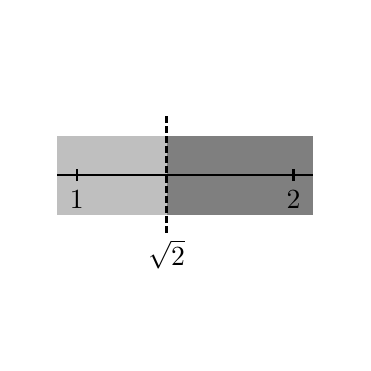
\begin{tikzpicture}[scale=0.5, font=\Large]
		\draw[draw=none] (-4,-4.25) -- (-4,3.75) -- (4,3.75) -- (4,-4.25) -- cycle;
		\draw[draw=none,fill=gray, fill opacity=0.5] (-3.25,-1) -- (-3.25,1) -- ({-2.75+5.5*(sqrt(2)-1)},1) --({-2.75+5.5*(sqrt(2)-1)},-1) -- cycle;
		\draw[draw=none,fill, fill opacity=0.5] ({-2.75+5.5*(sqrt(2)-1)},-1)--({-2.75+5.5*(sqrt(2)-1)},1) -- (3.25,1) -- ( 3.25,-1) -- cycle;
		\draw[thick] (-3.25,0) -- (3.25,0);
		\draw[thick] (-2.75,-0.15) -- (-2.75,0.15);
		\draw[thick] (2.75,-0.15) -- (2.75,0.15);
		\draw[thick, dash pattern=on 2.5pt off 1.1pt] ({-2.75+5.5*(sqrt(2)-1)},1.5) -- ({-2.75+5.5*(sqrt(2)-1)},-1.5);
		\tkzLabelPoint[below](-2.75,-0.15){$1$}
		\tkzLabelPoint[below](2.75,-0.15){$2$}
		\tkzLabelPoint[below]({-2.75+5.5*(sqrt(2)-1)},-1.4){$\sqrt{2}$}
	\end{tikzpicture}
\end{document}